\documentclass{article}

%\usepackage{mathtools}
\usepackage{amsfonts}
\usepackage[spanish,mexico]{babel}
\usepackage[utf8]{inputenc}
\usepackage{graphicx}
\usepackage{booktabs}
\usepackage{url}
\usepackage{listings}%http://www.tex.ac.uk/FAQ-codelist.html
\lstset{language=Python}
\graphicspath{ {img/} }
%\usepackage{enumitem}
%\usepackage{tikz}

\title{Representación mediante grafos de un problema de asignación de horarios}
\author{José Alberto Benavides Vázquez}
\date{\today}

\begin{document}

  \maketitle

  \section{Introducción}

  Los algoritmos de Floyd-Warshall y Ford-Fulkerson se utilizan en teoría de grafos para realizar mediciones de flujos a grafos ponderados. \textbf{Floyd-Warshall} calcula el camino más corto entre todos los pares de vértices, mientras que \textbf{Ford-Fulkerson} se utiliza para encontrar el máximo flujo que puede correr entre un nodo de inicio y uno de fin dados. Los nodos de inicio y fin de este segundo algoritmo se suelen denotar por $s$ y $t$ respectivamente.

  Este par de algoritmos se implementaron en un programa capaz de crear nodos, conectarlos y asignarles pesos y direcciones a las aristas así generadas. Este programa se halla alojado en \url{https://github.com/jbenavidesv87/FlujoRedes}.Se mostrará a continuación la explicación de dichos algoritmos además de ejecutarlos con un ejemplo para mayor claridad.

  \section{Ejecución}
  Tanto el algoritmo de Floyd-Warshall como el de Ford-Fulkerson toman un grafo previamente definido con al menos dos nodos conectados entre sí por una arista ponderada. Para demostrar el uso y funcionalidad de estos algoritmos, se construyó a manera de ejemplo un grafo $G$ no dirigido con cuatro nodos $a, b, c, d$, con aristas ponderadas como los mostrados en la figura \ref{fig:ejemplo} (p. \pageref{fig:ejemplo}).

  \begin{figure}[h]
    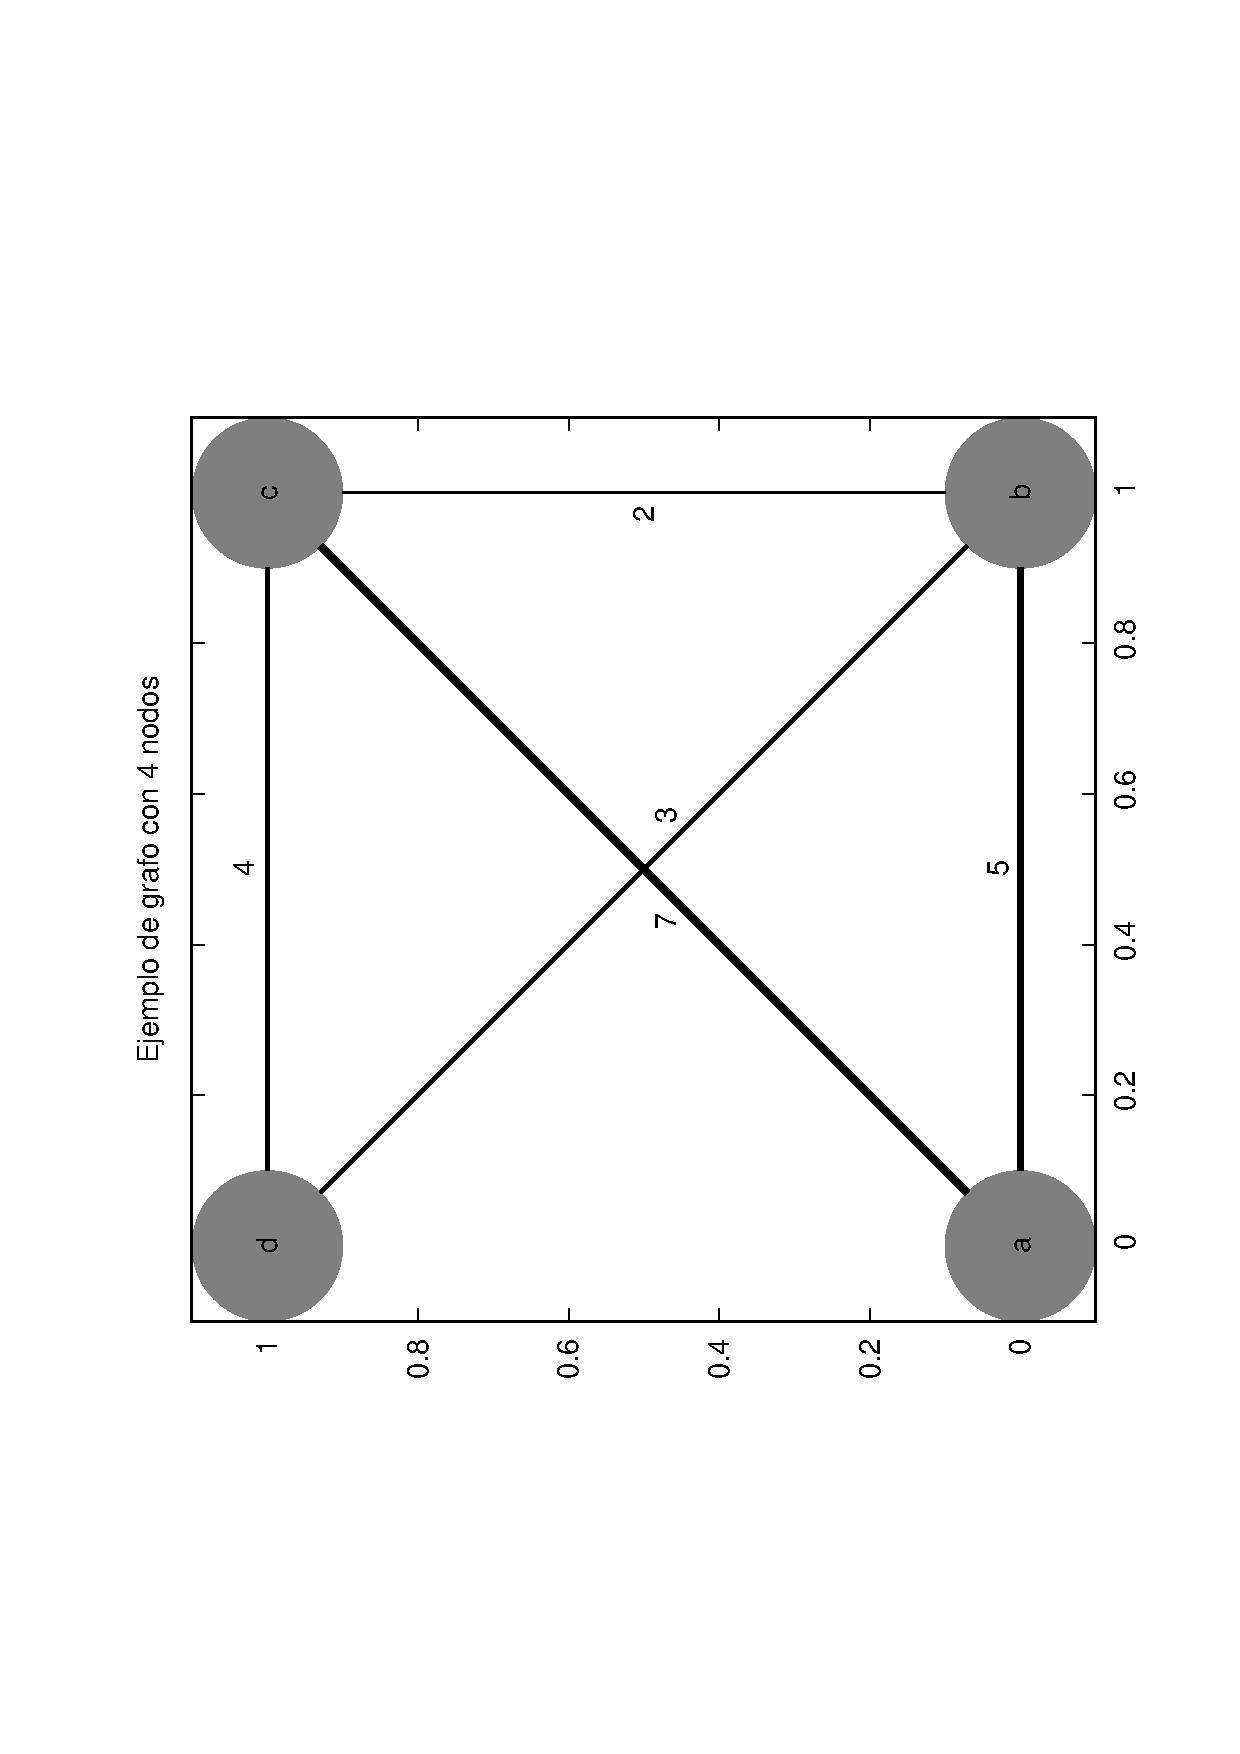
\includegraphics[width=0.7\textwidth, angle=-90]{ejemplo} % https://tex.stackexchange.com/questions/120117/how-to-rotate-eps-file
    \centering
    \caption{Grafo $G$ ponderado con 4 nodos $a, b, c, d$ que se usará como ejemplo para probar el funcionamiento de los algoritmos de Floyd-Warshall y Ford-Fulkerson.}
    \label{fig:ejemplo}
  \end{figure}

  % https://www.youtube.com/watch?v=4OQeCuLYj-4&t=186s
  Tras correr el algoritmo de Floyd-Warshal se obtuvieron, para cada par de nodos, el camino más corto entre todos los nodos del grafo. La distancia de estos caminos se calcula a partir de la suma de los pesos de las aristas que conectan a los nodos entre sí. En cada iteración, se exploran todos los caminos que van desde un nodo inicial hasta uno de destino. Se dice que un camino es mejor que otro cuando se encuentra un camino cuya distancia es menor a una existente (si no hay una distancia previamente almacenada, entonces se toma la primer distancia registrada como la mejor). Al final, el algoritmo regresa una lista de las mejores distancias entre todos los nodos. Para este ejemplo construido, la lista se puede consultar en el cuadro \ref{cuadro:floyd-ejemplo} (p. \pageref{cuadro:floyd-ejemplo}).

  \begin{table}[]
  \centering
  \caption{Camino más corto entre todos los pares de nodos, denotados por cada iteración como nodo inicial $s$ y nodo final $t$, para el grafo $G$ construido a manera de ejemplo inicial.}
  \label{cuadro:floyd-ejemplo}
  \begin{tabular}{@{}ccc@{}}
  \toprule
  \textbf{Nodo inicial $s$} & \textbf{Nodo final $t$} & \textbf{Camino más corto} \\ \midrule
  a & a & 0 \\ \midrule
  a & c & 7 \\ \midrule
  a & b & 5 \\ \midrule
  b & b & 0 \\ \midrule
  b & a & 5 \\ \midrule
  b & d & 3 \\ \midrule
  b & c & 2 \\ \midrule
  c & c & 0 \\ \midrule
  c & a & 7 \\ \midrule
  c & d & 4 \\ \midrule
  c & b & 2 \\ \midrule
  d & d & 0 \\ \midrule
  d & c & 4 \\ \midrule
  d & b & 3 \\ \midrule
  a & d & 8 \\ \midrule
  d & a & 8 \\ \bottomrule
  \end{tabular}
  \end{table}

  %https://www.youtube.com/watch?v=Tl90tNtKvxs
  El máximo flujo entre dos nodos se calcula con el algoritmo de Ford-Fulkerson. Este algoritmo consiste en recorrer todos los caminos que van desde un nodo inicial $s$ hasta uno final $f$, tomando como limitante el peso mínimo entre los pesos de los arcos que constituyen cada camino. Ese peso limitante indica el máximo flujo que podría soportar dicho camino. Cada iteración, se actualiza el grafo en el sentido en que se resta al peso de cada arco del camino elegido, el peso del camino mínimo. Cada iteración posterior, eligirá caminos en los que todos sus arcos posean capacidad disponible y se repite el proceso. Cuando no haya más caminos con arcos que tengan capacidades disponibles, se suman los pesos actualizados del grafo resultante, camino por camino, y se obtiene de su suma el máximo flujo del nodo $s$ al $t$. Del ejemplo graficado en la figura figura \ref{fig:ejemplo} (p. \pageref{fig:ejemplo}) se calculó el flujo máximo entre los nodos $a$ y $b$, obteniendo por resultado $10$; y entre los nodos $a$ y $d$, $7$.

  Ahora, este mismo algoritmo se correrá con el mismo grafo, pero dirigido, tal como se muestra en la figura \ref{fig:ejemploDirigido} (p. \pageref{fig:ejemploDirigido}). A este nuevo grafo se le llamará $H$.

  \begin{figure}[h]
    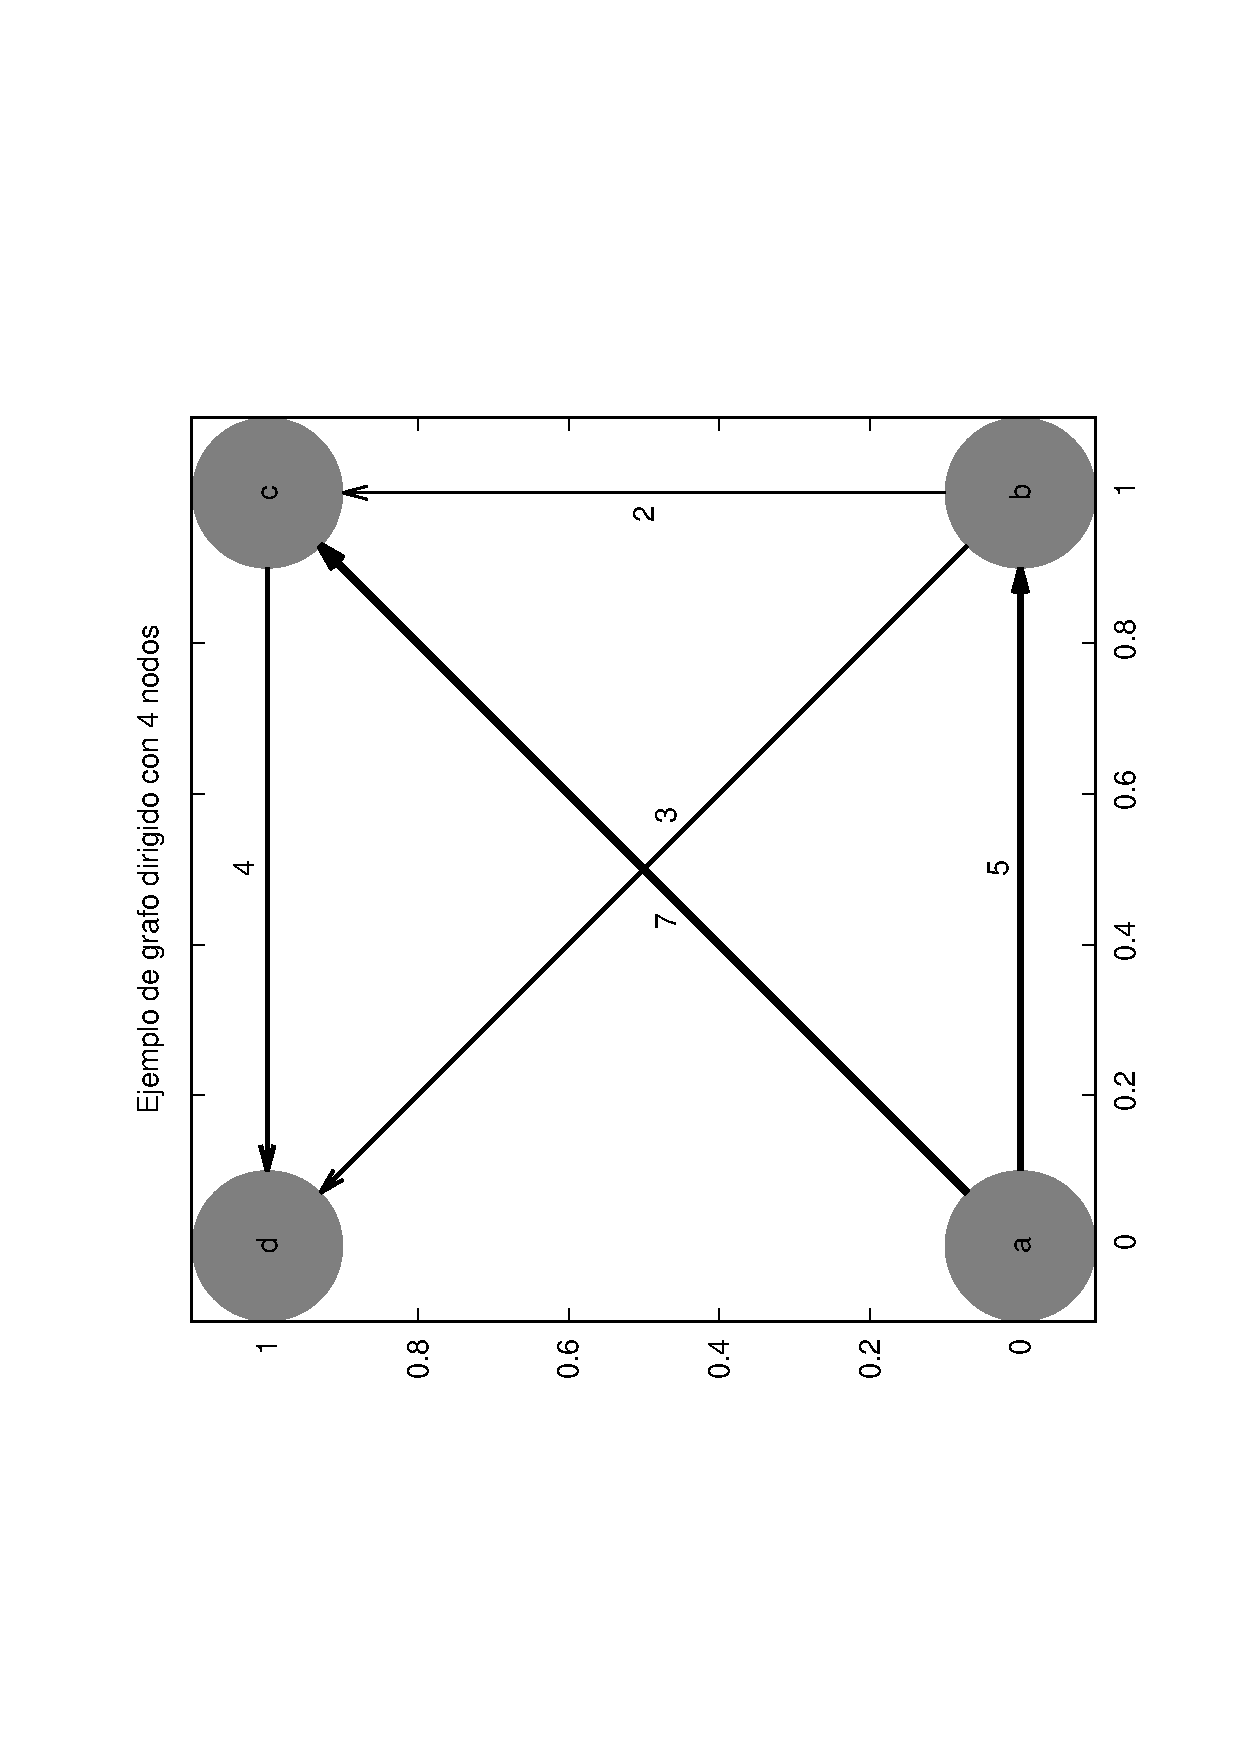
\includegraphics[width=0.7\textwidth, angle=-90]{ejemploDirigido} % https://tex.stackexchange.com/questions/120117/how-to-rotate-eps-file
    \centering
    \caption{Grafo $H$ ponderado y dirigido con 4 nodos $a, b, c, d$ que se usará como ejemplo para probar el funcionamiento de los algoritmos de Floyd-Warshall y Ford-Fulkerson.}
    \label{fig:ejemploDirigido}
  \end{figure}

  Tras correr el algoritmo de Floyd-Warshall en este

  %\bibliography{biblio}{}
  %\bibliographystyle{plain}

\end{document}
